\chapter{Implementasi Program dan Pengujian}

Pada bab ini, akan dijelaskan tentang lingkupan pembangunan, implementasi rancangan antarmuka, serta pengujian secara fungsional dan experimental pada aplikasi \textsl{data mining}.

\section{Lingkungan Pembangunan}
Lingkungan perangkat lunak dan perangkat keras yang digunakan untuk membangun dan menguji aplikasi \textsl{data mining} ini adalah:

\begin{enumerate}
	\item CPU
	\begin{itemize}
		\item Prosesor: Intel(R) Core(TM) i7, 1.60 GHz
		\item RAM: 6 GB
		\item VGA: NVDIA GeForce GT 330M
		\item Hardisk: 300 GB
	\end{itemize}
	\item Sistem operasi: Windows 7 Professional
	\item Platform: NetBeans: IDE 8.0
\end{enumerate}

\section{Hasil Tampilan Antarmuka}
Pada aplikasi \textsl{data mining} ini, terdapat dua form. Form pertama berfungsi untuk memilih file CSV yang akan dilakukan \textsl{data mining}, memilih metode pembuatan \textsl{decision tree}, serta menunjukkan hasil \textsl{decision tree} yang dihasilkan dalam bentuk String. Sedangkan untuk form kedua, berfungsi untuk memvisualisasikan \textsl{decision tree} yang sudah diperoleh dalam bentuk gambar.

TextField yang pertama berfungsi untuk mengisi alamat file CSV yang akan dilakukan \textsl{data mining}. RadioButton berfungsi untuk memilih metode manakah yang akan digunakan untuk membuat \textsl{decision tree}, sedangkan TextArea digunakan untuk memperlihatkan hasil \textsl{decision tree} dalam bentuk String. Tampilan awal aplikasi dapat dilihat di \ref{fig:GUI1}.

\begin{figure}[H]
\centering
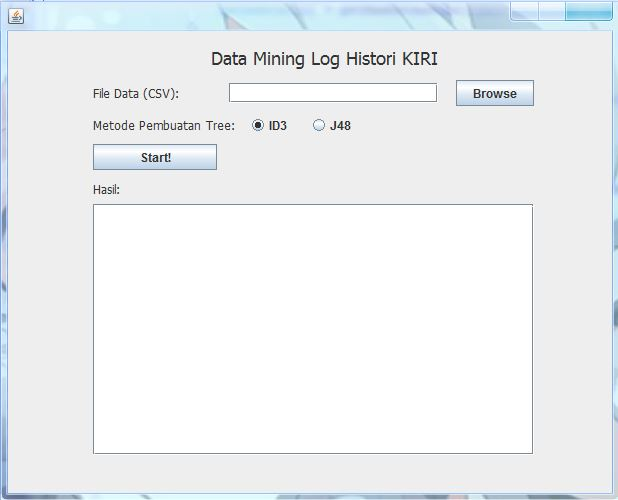
\includegraphics[scale=0.7]{Gambar/GUI1.jpg}
\caption[Tampilan Form Awal Aplikasi \textsl{Data Mining}]{Tampilan Form Awal Aplikasi \textsl{Data Mining}} 
\label{fig:GUI1}
\end{figure}

Terdapat dua cara untuk mengisi TextField, yaitu ditulis secara manual alamat file CSV atau dengan cara mengklik tombol button browse dan memilih file CSV pada FileSelector. Tampilan memilih file CSV dapat dilihat pada gambar \ref{fig:GUI2} dan tampilan setelah memilih file CSV dapat dilihat pada gambar \ref{fig:GUI3}.

\begin{figure}[H]
\centering
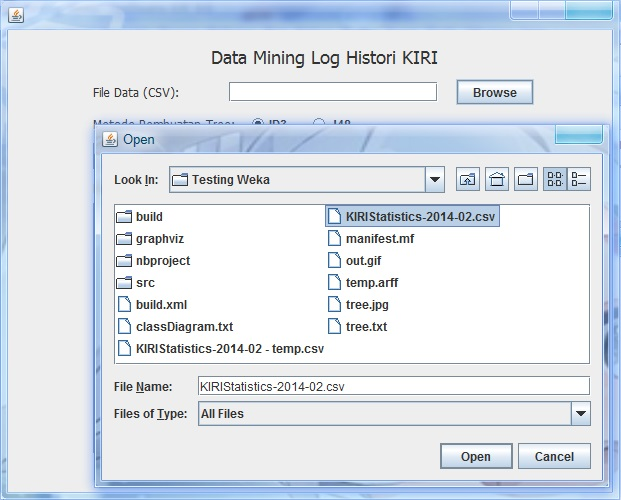
\includegraphics[scale=0.7]{Gambar/GUI2.jpg}
\caption[Tampilan FileSelector untuk Memilih File CSV]{Tampilan FileSelector untuk Memilih File CSV} 
\label{fig:GUI2}
\end{figure}

\begin{figure}[H]
\centering
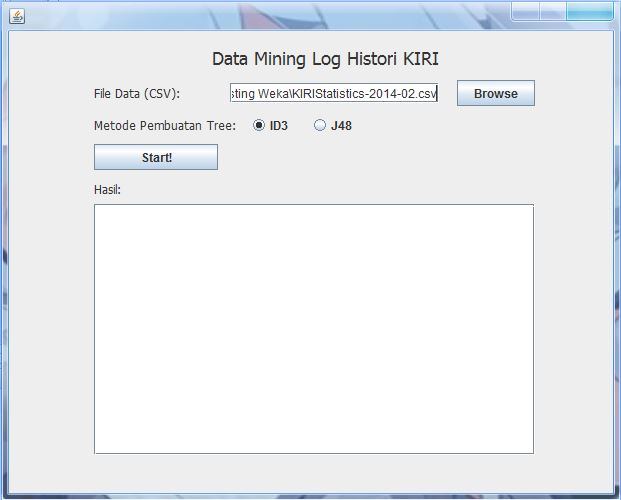
\includegraphics[scale=0.7]{Gambar/GUI3.jpg}
\caption[Tampilan Form setelah Memilih File CSV]{Tampilan Form setelah Memilih File CSV} 
\label{fig:GUI3}
\end{figure}

Setelah alamat file CSV diisi, hal selanjutnya yang dilakukan adalah memilih metode pembuatan \textsl{decision tree} pada RadioButton. RadioButton akan memilih metode ID3 jika \textsl{setting} ini tidak diubah. Tampilan tersebut dapat dilihat di gambar \ref{fig:GUI3and4}.

\begin{figure}[H]
\centering
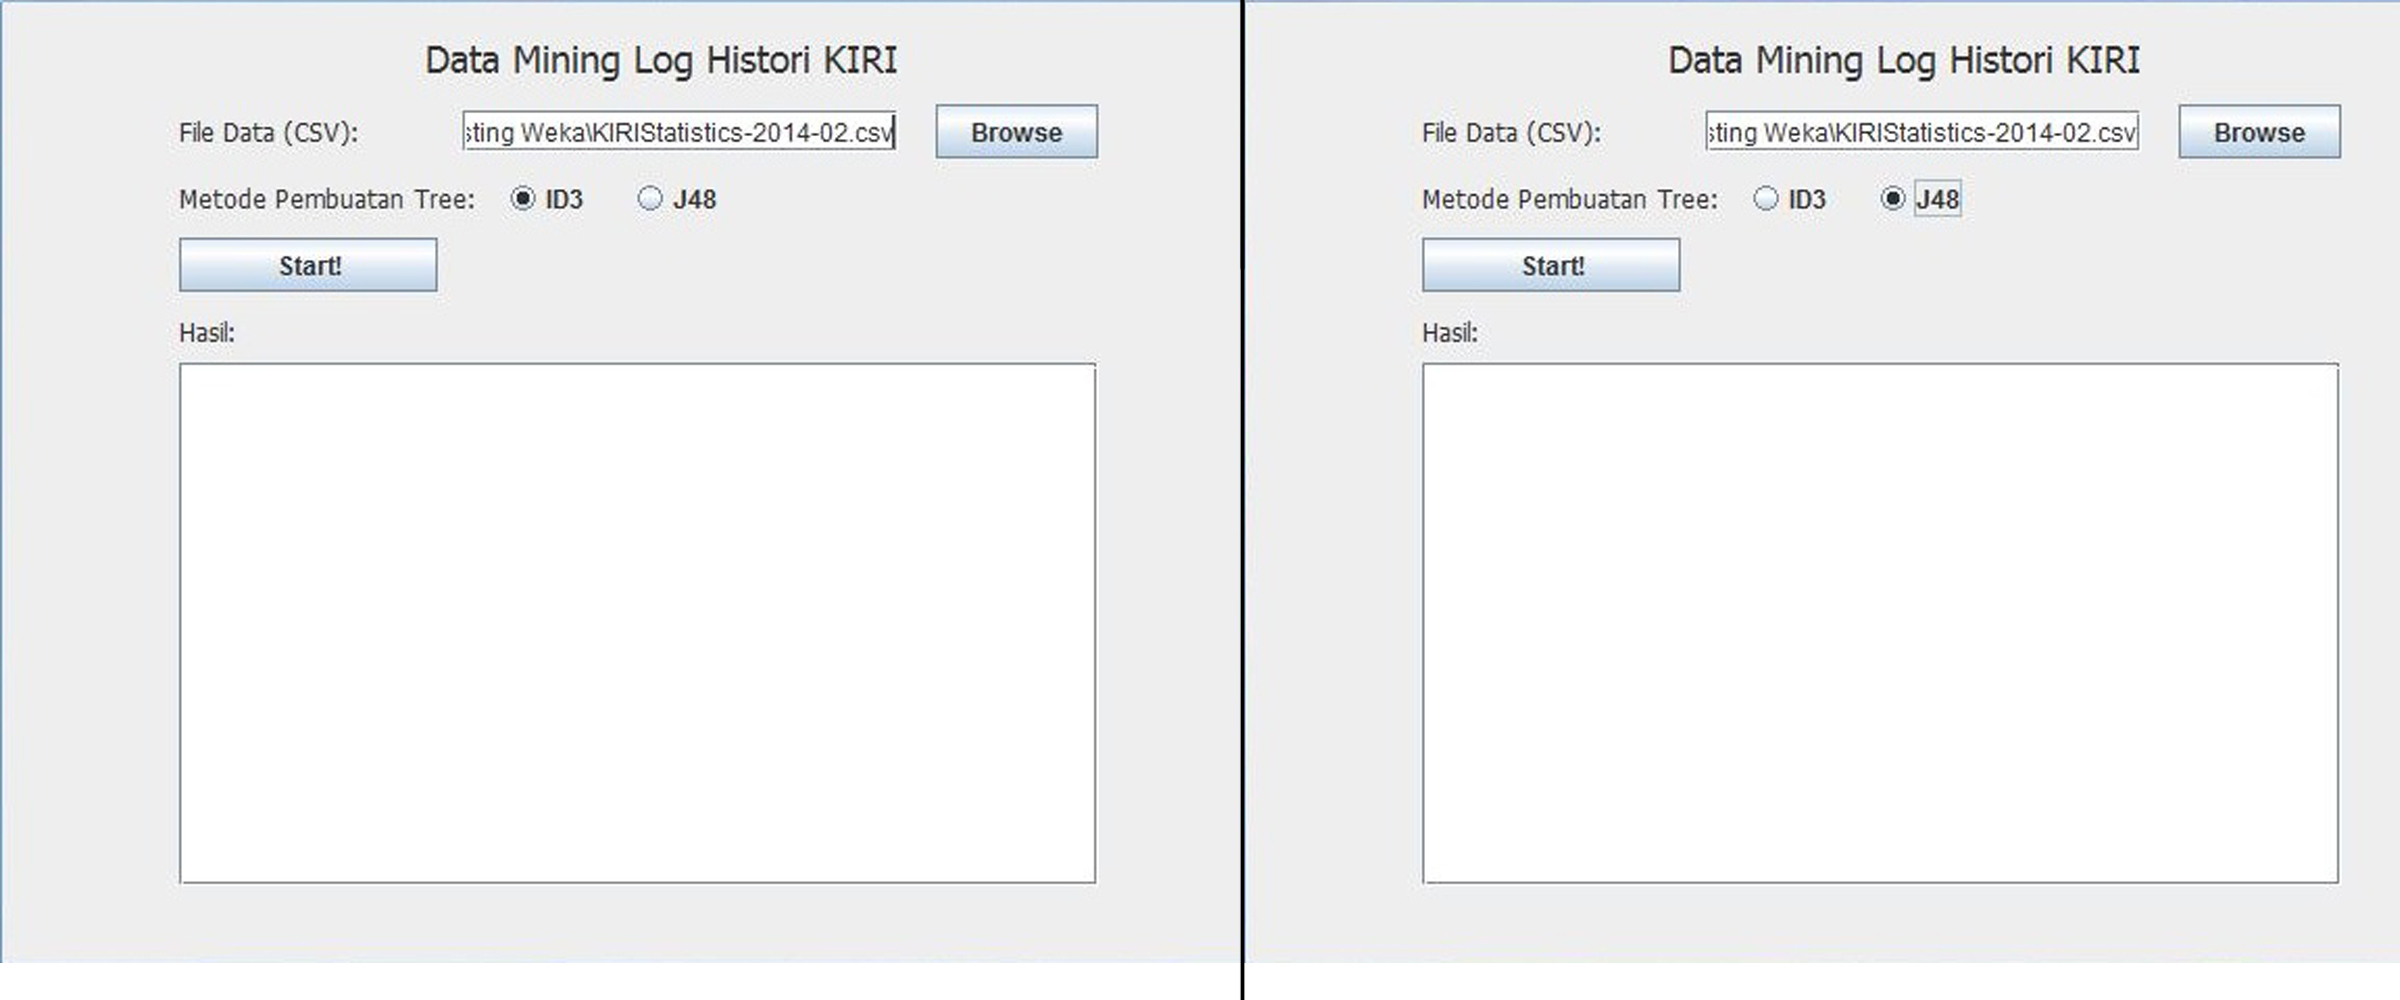
\includegraphics[scale=0.7]{Gambar/GUI3and4.jpg}
\caption[Tampilan Form Pemilihan Metode Pembuatan \textsl{Decision Tree}]{Tampilan Form Pemilihan Metode Pembuatan \textsl{Decision Tree}. Gambar a merupakan kondisi tampilan ketika metode ID3 dipilih sedangkan gambar b merupakan kondisi tampilan ketika metode J48 dipilih.} 
\label{fig:GUI3and4}
\end{figure}

Kemudian, tombol start diklik lalu program akan melakukan proses \textsl{data mining}. Setelah selesai, maka program akan menunjukkan hasil \textsl{data mining} dalam bentuk String pada TextArea dan dalam bentuk gambar pada form kedua. Tampilan akhir dari aplikasi serta form kedua dapat dilihat di gambar \ref{fig:GUI5}.

\begin{figure}[H]
\centering
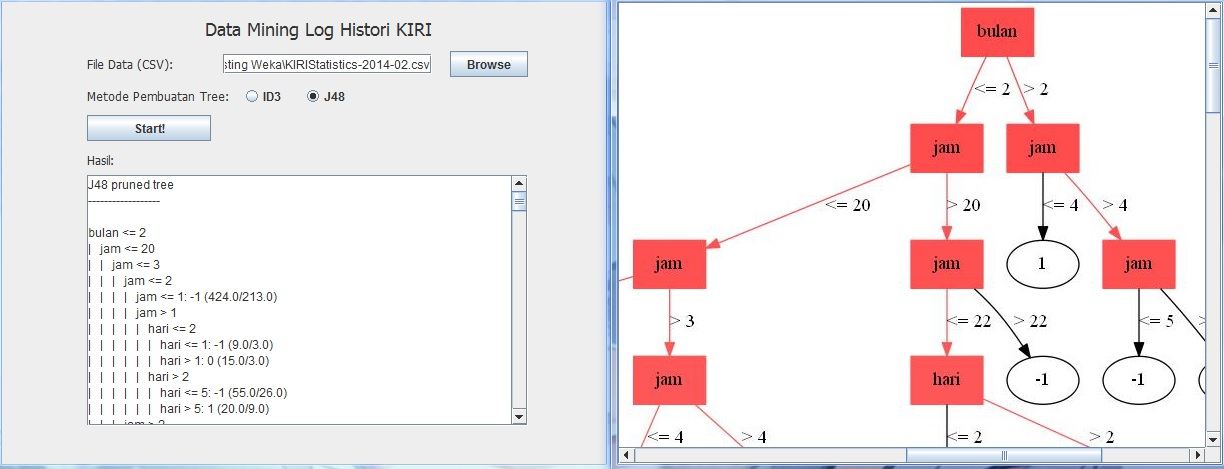
\includegraphics[scale=0.5]{Gambar/GUI5.jpg}
\caption[Tampilan Form Menampilkan Hasil \textsl{Data Mining}]{Tampilan Form Menampilkan Hasil \textsl{Data Mining}} 
\label{fig:GUI5}
\end{figure}

\section{Pengujian Aplikasi \textsl{Data Mining}}

\subsection{Pengujian Fungsional}

\subsubsection{Rancangan Pengujian}

Dalam pengujian aplikasi \textsl{data mining} ini, akan digunakan teknik pengujian \textsl{black box}. Pengujian yang akan dilakukan:
\begin{enumerate}
	\item Pengujian \textsl{method} utama untuk mencapai tujuan dari aplikasi \textsl{data mining} ini. Terdapat beberapa \textsl{method} yang perlu diuji, yaitu
	\begin{enumerate}
		\item \textsl{method} untuk membaca file CSV
		\item \textsl{method} untuk melakukan \textsl{preprocessing data}
		\item \textsl{method} untuk membuat \textsl{decision tree}
		\item \textsl{method} untuk mengubah \textsl{decision tree} dalam bentuk String menjadi bahasa DOT
	\end{enumerate}
	\item Kebenaran perangkat lunak hanya dilihat pada hasil keluaran program atau kondisi masukan yang diberikan tanpa melihat bagaimana proses untuk mendapatkan keluaran tersebut.
	\item Dari keluaran yang dihasilkan, kemampuan program untuk memenuhi kebutuhan pemakai dapat diukur dan dapat diketahui kesalahan jika ada.
\end{enumerate}


\subsubsection{Hasil Pengujian}

Dibuat sebuah \textsl{test case} yang berisi 20 data \textsl{log} histori KIRI dengan data pada tabel \ref{table:dataTestCase}

\begin{table}[H]
\rotatebox{90}{
\begin{tabular}{|l|l|l|l|l|}
\hline
\textbf{logId} & \textbf{APIKey}  & \textbf{Timestamp (UTC)} & \textbf{Action} & \textbf{AdditionalData}                                        \\ \hline
114055         & E5D9904F0A8B4F99 & 2/1/2014 2:34            & FINDROUTE       & -6.88968,107.59632/-6.88461,107.61361/3                        \\ \hline
114056         & E5D9904F0A8B4F99 & 2/1/2014 2:34            & FINDROUTE       & -6.88968,107.59632/-6.88461,107.61361/3                        \\ \hline
114057         & E5D9904F0A8B4F99 & 2/1/2014 2:34            & FINDROUTE       & -6.88968,107.59632/-6.88461,107.61361/3                        \\ \hline
114058         & A44EB361A179A49E & 2/1/2014 2:35            & FINDROUTE       & -6.9112484,107.6275648/-6.875449306549391,107.60455314069986/1 \\ \hline
114059         & E5D9904F0A8B4F99 & 2/1/2014 2:37            & PAGELOAD        & /5.10.83.99/                                                   \\ \hline
114060         & A44EB361A179A49E & 2/1/2014 2:38            & SEARCHPLACE     & cimol\%2C+/10                                                  \\ \hline
114061         & A44EB361A179A49E & 2/1/2014 2:38            & FINDROUTE       & -6.8779112,107.612129/-6.92663,107.63644/1                     \\ \hline
114062         & A44EB361A179A49E & 2/1/2014 2:38            & SEARCHPLACE     & gedebage\%2C+/10                                               \\ \hline
114063         & A44EB361A179A49E & 2/1/2014 2:38            & SEARCHPLACE     & gedebage\%2C+cimol/10                                          \\ \hline
114064         & A44EB361A179A49E & 2/1/2014 2:39            & FINDROUTE       & -7.3275023,108.3614085/-6.93269,107.69734/1                    \\ \hline
114065         & A44EB361A179A49E & 2/1/2014 2:39            & WIDGETLOAD      & /66.249.77.219/                                                \\ \hline
114066         & A44EB361A179A49E & 2/1/2014 2:39            & FINDROUTE       & -6.863680050774415,107.5951399281621/-6.93269,107.69734/1      \\ \hline
114067         & A44EB361A179A49E & 2/1/2014 2:43            & FINDROUTE       & -6.9423325,107.7486968/-6.90112,107.60787/1                    \\ \hline
114068         & A44EB361A179A49E & 2/1/2014 2:43            & FINDROUTE       & -6.9423325,107.7486968/-6.88623,107.60821/1                    \\ \hline
114069         & A44EB361A179A49E & 2/1/2014 2:44            & FINDROUTE       & -6.9423062,107.7490084/-6.88623,107.60821/1                    \\ \hline
114070         & A44EB361A179A49E & 2/1/2014 2:45            & FINDROUTE       & -6.9072888,107.6143937/-6.90855,107.61082/1                    \\ \hline
114071         & A44EB361A179A49E & 2/1/2014 2:46            & FINDROUTE       & -6.9286306,107.6227444/-6.91708,107.60880/1                    \\ \hline
114072         & A44EB361A179A49E & 2/1/2014 2:46            & FINDROUTE       & -6.908639785445589,107.61091567575932/-6.90855,107.61082/1     \\ \hline
114073         & A44EB361A179A49E & 2/1/2014 2:47            & SEARCHPLACE     & hotel+harapan+i/10                                             \\ \hline
114074         & A44EB361A179A49E & 2/1/2014 2:47            & SEARCHPLACE     & hotel+harapan+ind/10                                           \\ \hline
\end{tabular}}
\caption{Data untuk \textsl{Test Case} Aplikasi \textsl{Data Mining}}
\label{table:dataTestCase}
\end{table}

Berikut hasil pengujian yang dilakukan dengan menggunakan data tersebut:
\begin{enumerate}
	\item Pengujian pertama: Membaca file CSV, data akan diambil oleh program dan dipilah, hanya record dengan \textsl{action} FINDROUTE yang akan diambil sedangkan yang lain akan dibuang. Berikut hasil dengan contoh data diatas dengan menggunakan sistem \textsl{debug} untuk melihat data yang diambil dari CSV pada gambar \ref{fig:Pengujian1} dan \ref{fig:Pengujian12}
	
	\begin{figure}[H]
	\centering
	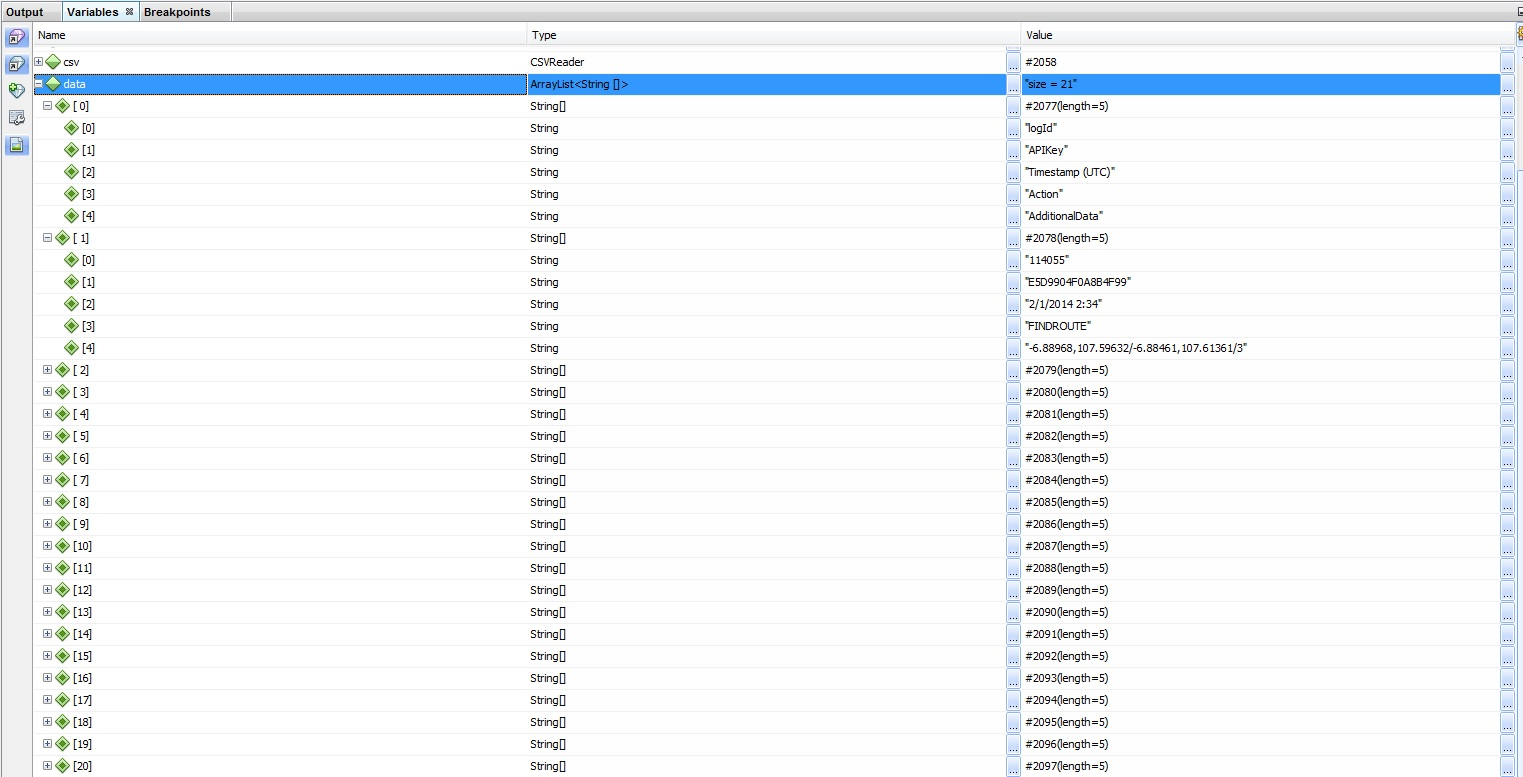
\includegraphics[scale=0.4]{Gambar/pengujian1.jpg}
	\caption[Pengujian Mengambil Data CSV]{Pengujian Mengambil Data CSV} 
	\label{fig:Pengujian1}
	\end{figure}

	\begin{figure}[H]
	\centering
	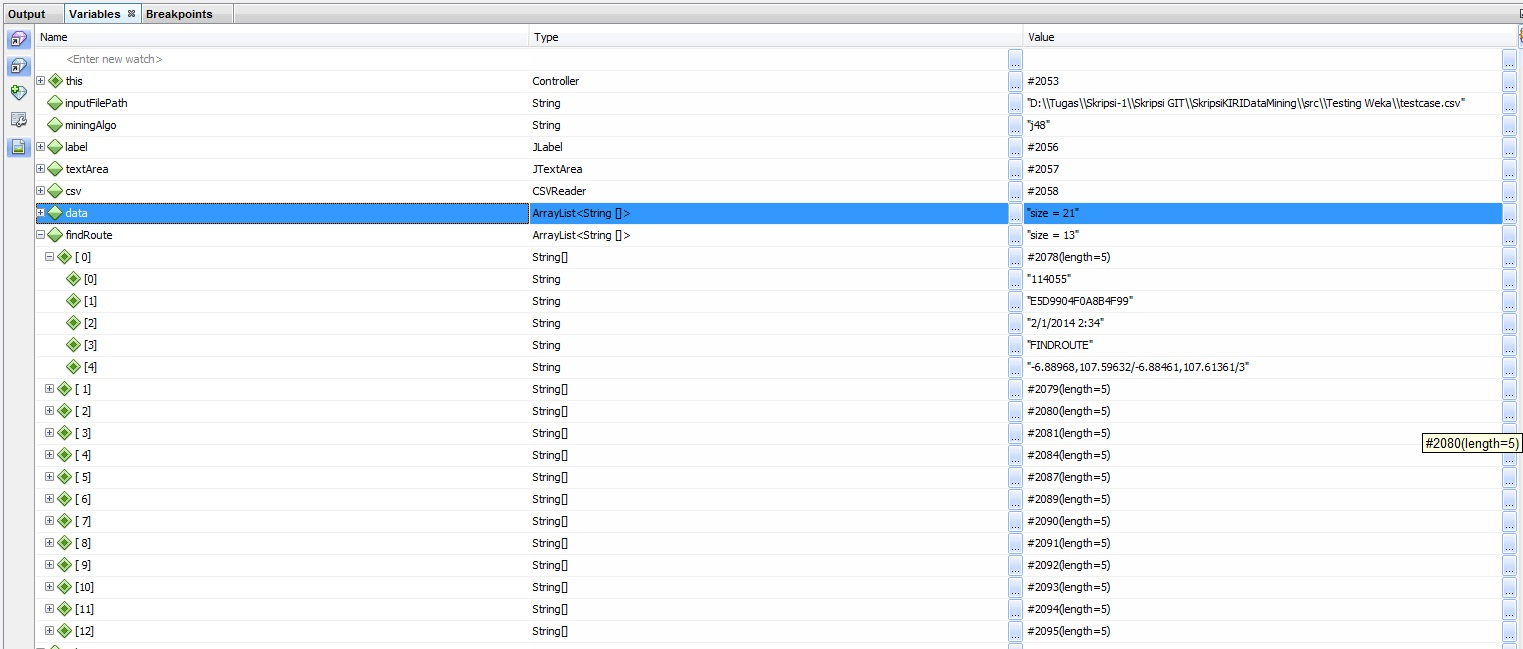
\includegraphics[scale=0.4]{Gambar/pengujian12.jpg}
	\caption[Pengujian \textsl{Data Selection} untuk Mengambil Data dengan \textsl{Action} FINDROUTE]{Pengujian \textsl{Data Selection} untuk Mengambil Data dengan \textsl{Action} FINDROUTE} 
	\label{fig:Pengujian12}
	\end{figure}

	Gambar pertama memperlihatkan bahwa data pertama yang diperoleh 21 array String dengan array pertama adalah atributnya sedangkan array selanjutnya adalah isi data yang diperoleh. Pada gambar kedua, terdapat 13 array String dimana semua array tersebut merupakan record dengan nilai \textsl{action} FINDROUTE saja. Dengan demikian, pengujian membaca CSV berhasil dilakukan.

	\item Pengujian kedua: Melakukan \textsl{preprocessing data}, data yang digunakan adalah 13 array String yang sudah diperoleh dari pengujian pertama. Pengujian dilakukan dengan melakukan pengecekan data dengan menggunakan weka untuk melihat data yang sudah dihasilkan, dapat dilihat pada \ref{fig:Pengujian214} dan \ref{fig:Pengujian25} 
	
	\begin{figure}[H]
	\centering
	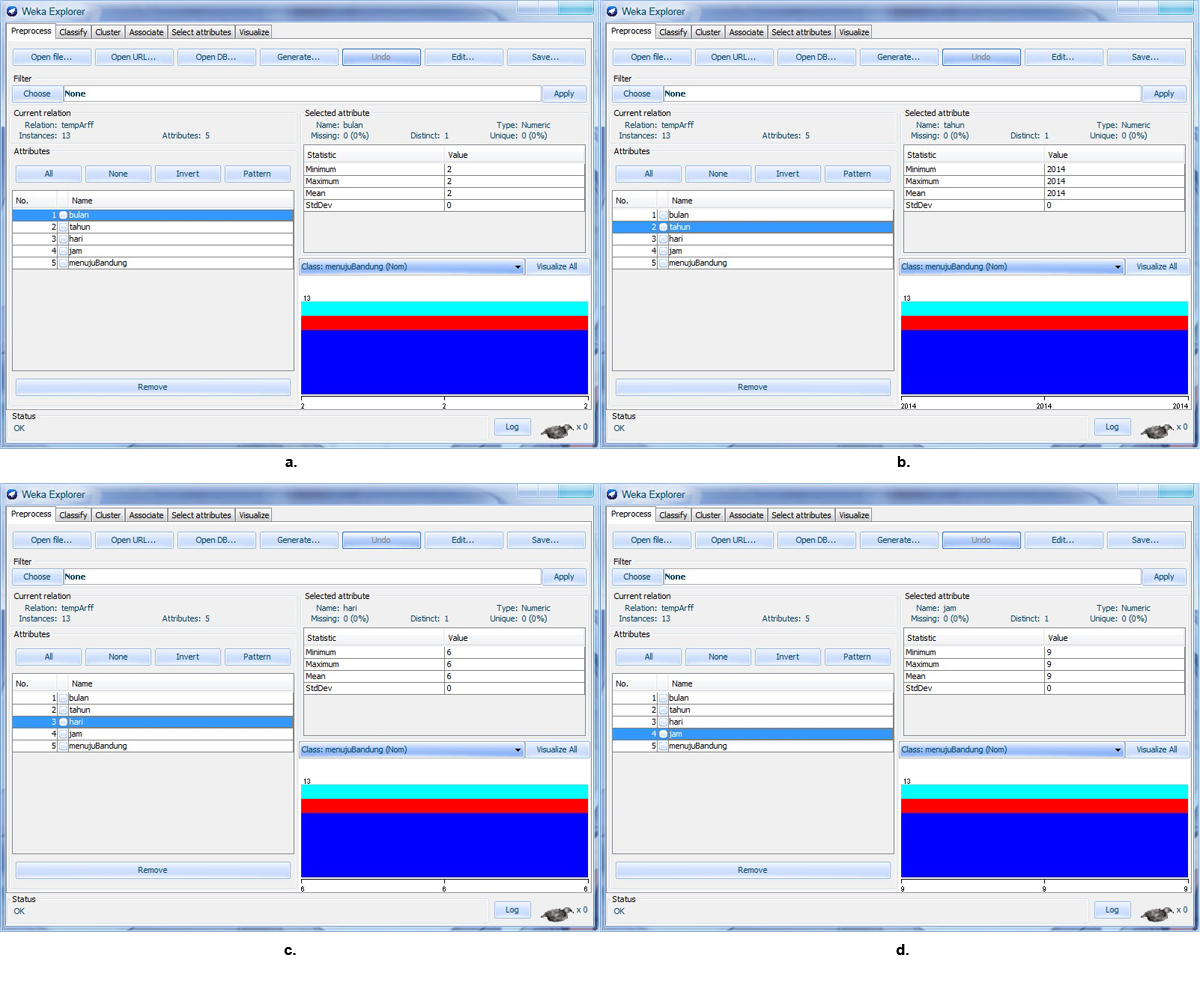
\includegraphics[scale=0.4]{Gambar/pengujian214.jpg}
	\caption[Pengujian \textsl{Preprocessing Data}]{Pengujian \textsl{Preprocessing Data}. Gambar a menunjukkan nilai pada atribut bulan. Gambar b menunjukkan nilai pada atribut tahun. Gambar c menunjukkan nilai pada atribut hari. Gambar d menunjukkan nilai pada atribut jam.} 
	\label{fig:Pengujian214}
	\end{figure}
	
	\begin{figure}[H]
	\centering
	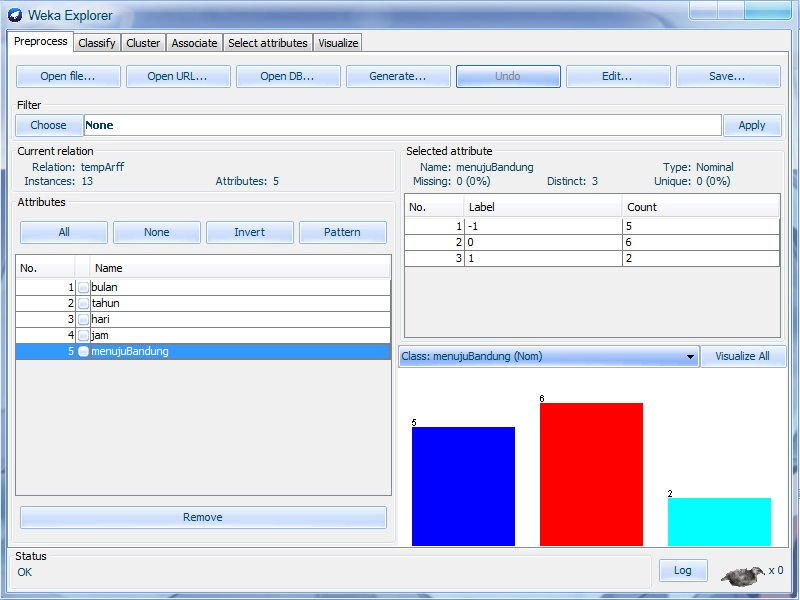
\includegraphics[scale=0.4]{Gambar/pengujian25.jpg}
	\caption[Pengujian \textsl{Preprocessing Data} untuk Klasifikasi Data]{Pengujian \textsl{Preprocessing Data} untuk Klasifikasi Data} 
	\label{fig:Pengujian25}
	\end{figure}

	Terdapat dua tahap penting pada \textsl{prerpocessing data}, yaitu pengubahan waktu dari UTC menjadi GMT+7 dan klasifikasi area. Pada tahap pengubahan waktu dari UTC menjadi GMT+7, pada gambar \ref{fig:Pengujian214} d, atribut jam yang dimiliki menjadi bernilai sembilan karena pada testcase, nilai atribut jam adalah dua. Pada tahap klasifikasi area, dapat dilihat pada tabel \ref{table:PenentuanAreaDanKlasifikasi}
	
	\begin{table}[H]
	\centering
	\begin{tabular}{|l|l|l|}
	\hline
	\multicolumn{1}{|c|}{\textbf{Region Keberangkatan}} & \multicolumn{1}{c|}{\textbf{Region Tujuan}} & \multicolumn{1}{c|}{\textbf{Hasil Klasifikasi}} \\ \hline
	3                                                   & 3                                           & 0                                               \\ \hline
	3                                                   & 3                                           & 0                                               \\ \hline
	3                                                   & 3                                           & 0                                               \\ \hline
	3                                                   & 4                                           & 1                                               \\ \hline
	4                                                   & 4                                           & 0                                               \\ \hline
	11                                                  & 10                                          & -1                                              \\ \hline
	5                                                   & 10                                          & 1                                               \\ \hline
	11                                                  & 1                                           & -1                                              \\ \hline
	11                                                  & 3                                           & -1                                              \\ \hline
	11                                                  & 3                                           & -1                                              \\ \hline
	1                                                   & 1                                           & 0                                               \\ \hline
	2                                                   & 0                                           & -1                                              \\ \hline
	1                                                   & 1                                           & 0                                               \\ \hline
	\end{tabular}
	\caption{Hasil Penentuan area dan Klasifikasi}
	\label{table:PenentuanAreaDanKlasifikasi}
	\end{table}
	
	Terdapat lima data dengan klasifikasi -1, enam data dengan klasifikasi 0, dan 2 data dengan klasifikasi 1. Dari kedua hasil tersebut, dapat disimpulkan bahwa tahap \textsl{preprocessing data} sudah berjalan dengan baik.
	
	\item Pengujian ketiga: Membuat \textsl{decision tree}, akan dilakukan perbandingan antara hasil dari program dengan hasil dari weka, dapat dilihat pada gambar \ref{fig:Pengujian31} dan 
	\ref{fig:Pengujian32}.
	
	\begin{figure}[H]
	\centering
	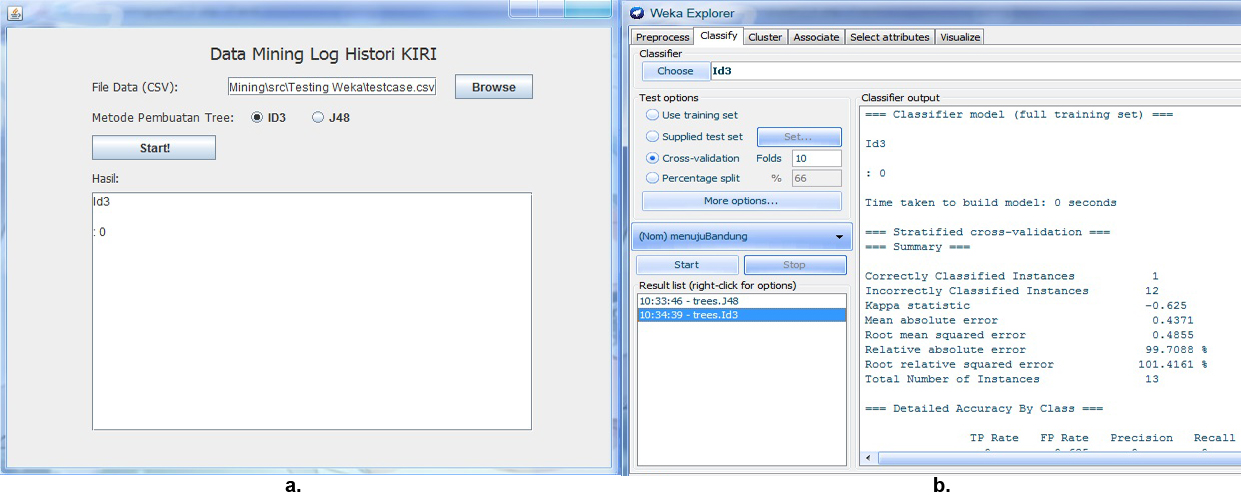
\includegraphics[scale=0.4]{Gambar/pengujian31.jpg}
	\caption[Pengujian Pembuatan \textsl{Decision Tree} ID3]{Pengujian Pembuatan \textsl{Decision Tree} ID3. Gambar a merupakan hasil dari aplikasi \textsl{data mining} sedangkan gambar b merupakan hasil dari weka.} 
	\label{fig:Pengujian31}
	\end{figure}

	\begin{figure}[H]
	\centering
	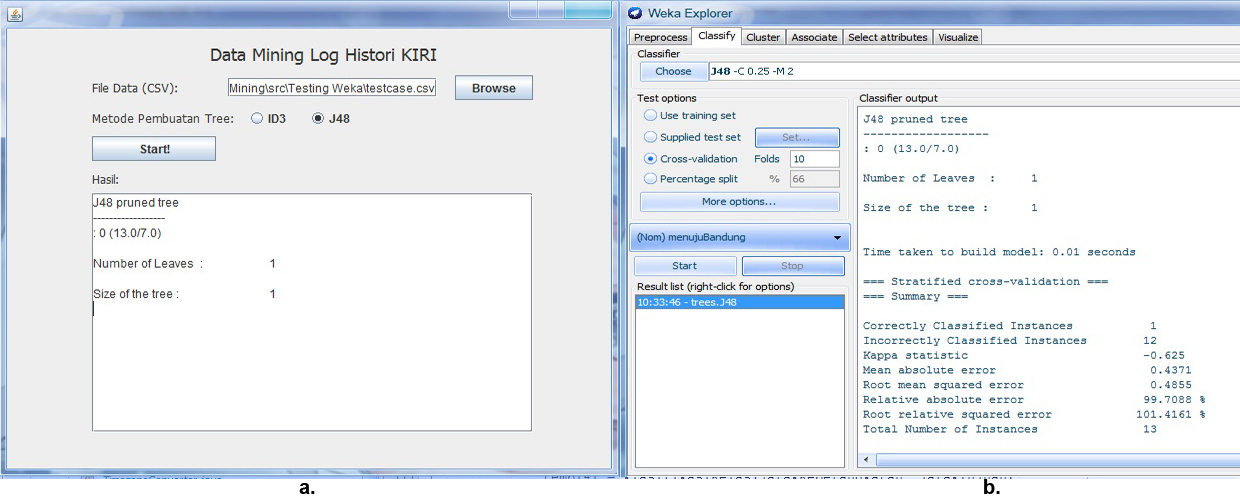
\includegraphics[scale=0.4]{Gambar/pengujian32.jpg}
	\caption[Pengujian Pembuatan \textsl{Decision Tree} J48]{Pengujian  Pembuatan \textsl{Decision Tree} J48. Gambar a merupakan hasil dari aplikasi \textsl{data mining} sedangkan gambar b merupakan hasil dari weka.} 
	\label{fig:Pengujian32}
	\end{figure}

	Dari kedua gambar tersebut, dapat disimpulkan bahwa hasil \textsl{decision tree} yang dihasilkan sama dan benar.
	
	\item Pengujian keempat: Mengubah \textsl{decision tree} dalam bentuk String menjadi bahasa DOT, akan dilakukan visualisasi \textsl{decision tree} dengan membuat graph dalam bahasa DOT, dapat dilihat pada gambar \ref{fig:Pengujian4}.
	
	\begin{figure}[H]
	\centering
	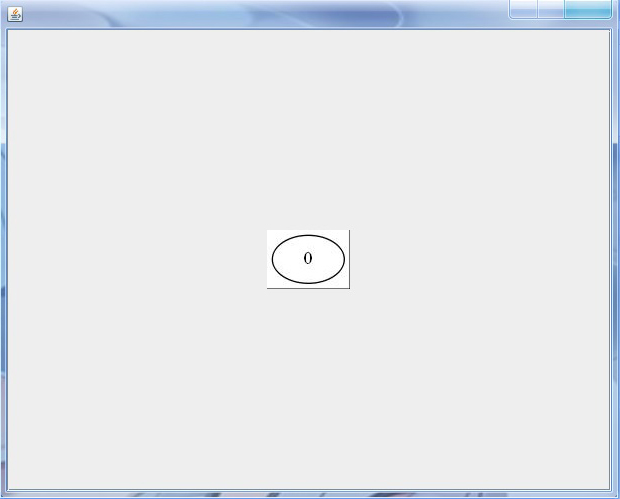
\includegraphics[scale=0.4]{Gambar/pengujian4.jpg}
	\caption[Pengujian Hasil Visualisasi dengan Menggunakan Bahasa DOT]{Pengujian Hasil Visualisasi dengan Menggunakan Bahasa DOT.} 
	\label{fig:Pengujian4}
	\end{figure}
	
	Dari gambar tersebut, dapat disimpulkan bahwa pengubahan \textsl{decision tree} menjadi bahasa DOT telah berhasil.

\end{enumerate}

\subsection{Pengujian Eksperimental}

Pada subbab ini, akan dilakukan pengujian pada data 1 bulan dari \textsl{log} histori KIRI pada bulan Febuari.

Ketika Pengujian dilakukan, ditemukan \textsl{bug} data yaitu terdapat nilai dari data \textsl{log} histori KIRI pada \textsl{action} FINDROUTE kolom additionalData dengan format String yang berbeda. Kesalahan format tersebut adalah nilai pembatas angka dibelakang koma yang seharusnya menggunakan titik menjadi koma, sehingga pemotongan nilai String menghasilkan data yang salah dan \textsl{error}. Dari pengujian ini, maka diperlukan \textsl{data cleaning} pada tahap \textsl{preprocessing data} agar data dengan format yang salah dapat dibuang dan tidak menyebabkan \textsl{error}. Hasil error yang ditemukan dari \textsl{data cleaning} dapat dilihat pada gambar \ref{fig:percobaanError}.

\begin{figure}[H]
\centering
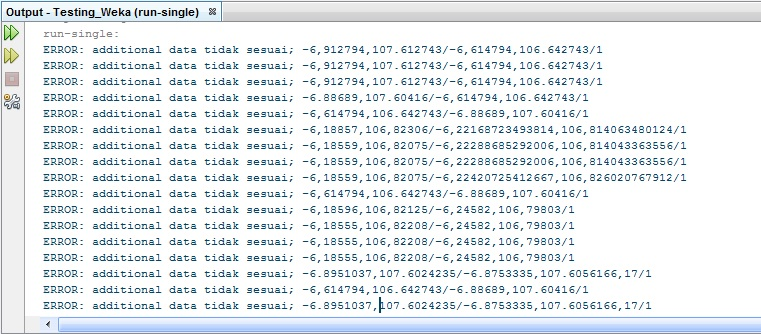
\includegraphics[scale=0.5]{Gambar/percobaanError.jpg}
\caption[Percobaan \textsl{Data Mining} untuk Melakukan Data Cleaning]{Percobaan \textsl{Data Mining} untuk Melakukan Data Cleaning.} 
\label{fig:percobaanError}
\end{figure}

Setelah melakukan \textsl{data cleaning}, program dapat berjalan dengan baik. Berikut hasil dari percobaan metode ID3 pada gambar \ref{fig:percobaan1} dan metode J48 pada gambar \ref{fig:percobaan2}.

\begin{figure}[H]
\centering
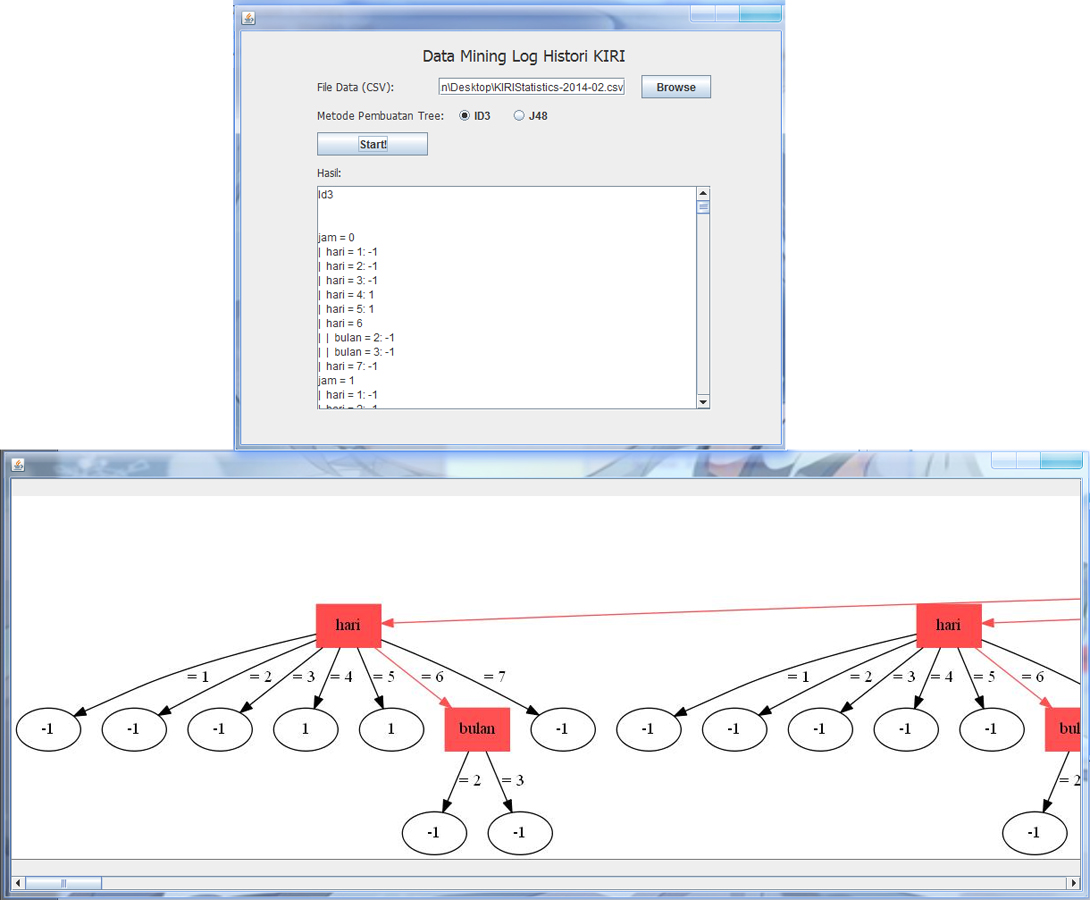
\includegraphics[scale=0.5]{Gambar/percobaan1.jpg}
\caption[Percobaan \textsl{Data Mining} dengan Menggunakan Metode ID3 pada \textsl{Log} Histori KIRI pada Bulan 2 Tahun 2014]{Percobaan \textsl{Data Mining} dengan Menggunakan Metode ID3 pada \textsl{Log} Histori KIRI pada Bulan 2 Tahun 2014.} 
\label{fig:percobaan1}
\end{figure}

\begin{figure}[H]
\centering
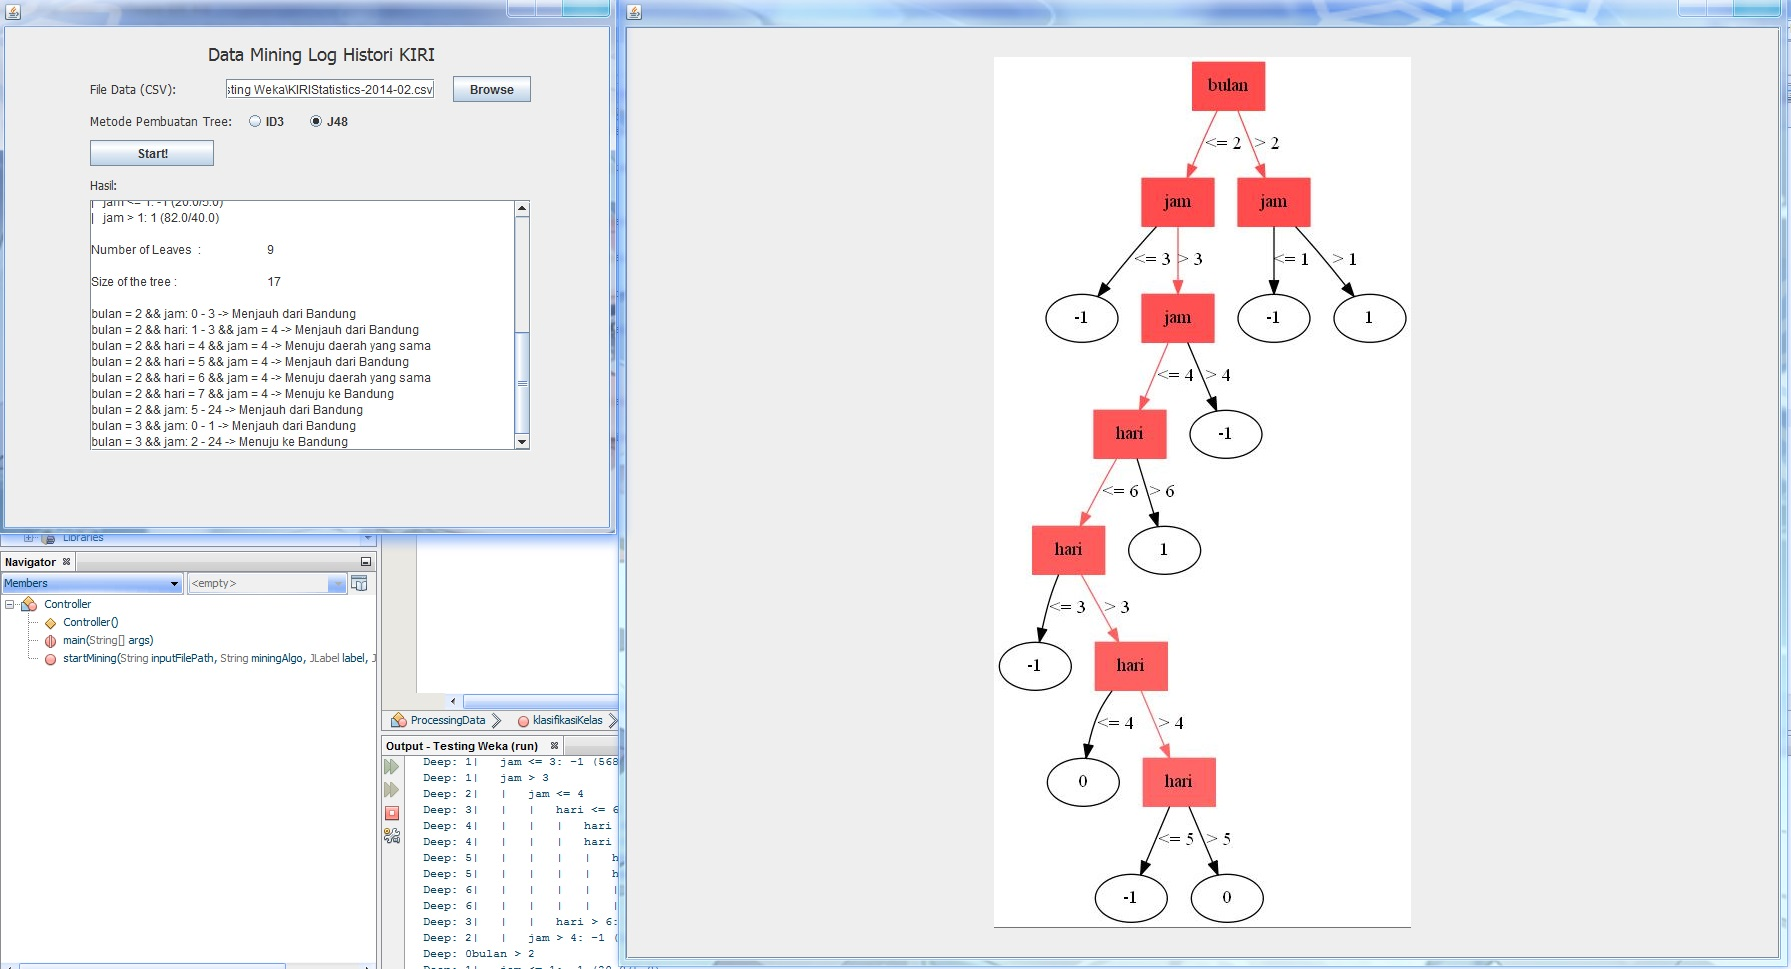
\includegraphics[scale=0.3]{Gambar/percobaan2.jpg}
\caption[Percobaan \textsl{Data Mining} dengan Menggunakan Metode J48 pada \textsl{Log} Histori KIRI pada Bulan 2 Tahun 2014]{Percobaan \textsl{Data Mining} dengan Menggunakan Metode J48 pada \textsl{Log} Histori KIRI pada Bulan 2 Tahun 2014.} 
\label{fig:percobaan2}
\end{figure}

Pada kedua percobaan, terdapat perbedaan bulan, hal ini dikarenakan perubahan waktu dari UTC menuju GMT+7 sehingga terdapat perubahan bulan atau tahun. Karena data pada bulan selanjutnya hanya tujuh jam, maka hasil pada bulan selanjutnya lebih baik tidak dianggap karena data tersebut tidak cukup untuk merepresentasikan waktu satu bulan.

Hasil percobaan pembuatan \textsl{decision tree} pada metode ID3 mengalami overfitting karena menghasilkan klasifikasi pada hampir setiap kemungkinan, dapat disimpulkan hasil \textsl{decision tree} pada percobaan di bulan ini cukup jelek. Namun pada percobaan metode J48, menghasilkan \textsl{decision tree} yang tidak overfitting dan menarik dimana dinyatakan bahwa jam 0-3 dan jam 5-24 user menjauhi Bandung.

Nilai akurasi dari percobaan dengan metode ID3 adalah 35.65\% sedangkan untuk percobaan dengan metode j48 adalah 47.33\%, dari sini dapat dinyatakan bahwa hasil \textsl{decision tree} dari j48 lebih tepat daripada ID3 namun kedua metode tersebut menghasilkan nilai akurasi yang belum memuaskan, karena masih dibawah 50\%


Selain itu, dari kedua percobaan ini, diperoleh bahwa cukup sulit untuk membaca hasil \textsl{decision tree} terutama pada \textsl{node} dengan kedalaman lebih dari 4 tingkat. Oleh karena itu, akan ditambahkan fungsi agar \textsl{decision tree} lebih mudah dibaca. Program akan ditambah satu kelas baru yaitu SDForExtractData yang berfungsi untuk menyimpan data dan membuat kesimpulan dari setiap \textsl{leaf} yang dihasilkan.

Berikut hasil dari fungsi yang dibuat agar \textsl{decision tree} lebih mudah dibaca, dapat dilihat pada gambar \ref{fig:percobaan3}.

\begin{figure}[H]
\centering
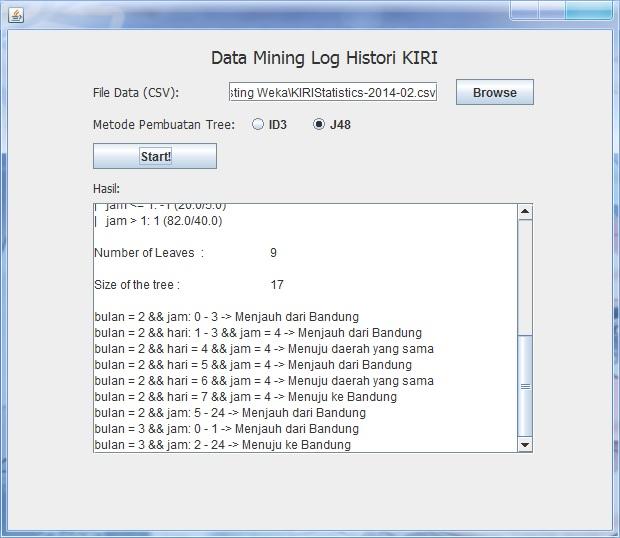
\includegraphics[scale=0.7]{Gambar/percobaan3.jpg}
\caption[Hasil dari SDForExtractData]{Hasil dari SDForExtractData} 
\label{fig:percobaan3}
\end{figure}

Dengan fungsi tersebut, diharapkan user dapat lebih mudah membaca \textsl{decision tree} yang dihasilkan.

\subsection{Analisis Hasil Uji}

Berdasarkan pengujian di atas, dapat disimpulkan bahwa 

\begin{enumerate}
	\item Metode ID3 menghasilkan \textsl{decision tree} yang bersifat overfitting.
	\item Metode J48 menghasilkan \textsl{decision tree} yang lebih baik dan tepat daripada ID3, khususnya pada data \textsl{log} histori KIRI dengan \textsl{preprocessing data} dan klasifikasi yang sudah dijelaskan pada bab 3 (J48 menghasilkan 43\% sedangkan ID3 menghasilkan 36.55\%).
	\item Kedua metode belum menghasilkan nilai akurasi yang memuaskan, karena masih dibawah 50\%.
	\item Dari data \textsl{log} histori KIRI pada bulan Febuari 2014, \textsl{decision tree} dengan metode J48 menyatakan bahwa penduduk Bandung lebih sering menjauhi Bandung jika dilihat dari banyak jam dimana user menjauhi Bandung.
\end{enumerate}













